\scanpage{86}
\mspage{85}
\mspage{\handwritten{18}}
\mspage{\deleted{\handwritten{16}}}
\margin{\handwritten{\figure{\begin{tikzpicture}[x=.12cm,y=.12cm]
\draw[line width=.6pt] (0,1.55)--(-.04,1.25);
\draw[line width=.4pt] (-.08,.8)--(-.12,-.2);
\end{tikzpicture}}}}
2.7\rlap{\handwritten{\begin{tikzpicture}[baseline=0cm,x=1cm,y=1cm]\draw[thin] (.04,.02)--(.05,.27);\end{tikzpicture}}}. \handwritten{\uline}{Topos classifiant d'un \inserted{\handwritten{pro-}}\handwritten{\begin{tikzpicture}[baseline=0cm,x=1cm,y=1cm]\draw[thin] (0,-.15)..controls (.05,.08) and (.1,.18)..(.35,.2)--(.8,.24);\end{tikzpicture}}groupe\handwritten{.} \deleted{profini}.}

\handwritten{\begin{tikzpicture}[baseline=0cm]\fill (0,0) circle (.018cm);\end{tikzpicture}}\handwritten{2.7.1} Soit $\inserted{\handwritten{\underline}{G}=}(G_i)_{i\handwritten{\in}I}$ un syst\rlap{p}ê\rlap{e}me projectif \deleted{strict} de groupes, avec $G_i,I\handwritten{\in}\handwritten{\underline}{U}$. On suppose le systême projectif \handwritten{\uline}{strict}, i.e. les morphismes de transition $G_j\handwritten{\to}G_i$ surjectifs. \margin{\handwritten{\figure{\begin{tikzpicture}[x=.3cm,y=.3cm]
\draw (0,.15) .. controls (.2,-.05) and (.4,-.25) .. (.65,-.2);
\end{tikzpicture}}}}Si $E$ est un e\rlap{s}n\rlap{n}semble, on \deleted{dit que $\handwritten{\underline}{G}$ \handwritten{\uline}{opère} sur $E$} \deleted{si} appelle \handwritten{\uline}{opération de} $\handwritten{\underline}{G}$ \handwritten{\uline}{sur} $E$\inserted{(à gauche, disons\unsure{\rlap{p}\handwritten{)}|)\handwritten{)}}}\handwritten{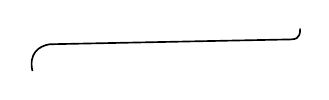
\begin{tikzpicture}[baseline=0cm,x=1cm,y=1cm]\draw[semithick] (0,-.17)..controls (-.05,.05) and (.08,.15)..(.22,.17)--(3.2,.23)..controls (3.35,.23) and (3.4,.23)..(3.4,.37);\end{tikzpicture}} la structure suivante: a) une famille $(E_i)_{i\handwritten{\in}I}$ de parties de $E$, de réunion $E$; b) pour tout $i\handwritten{\in}I$, une opération du groupe $G_i$ sur l'ensemble $E_i$ ; on suppose de plus ces données soumises à la condition suivante: pour $j\handwritten{\geq}i$, $E_i$ est le sous-ensemble de $E_j$ formé des éléments fixes sous le groupe noyau de $G_j\handwritten{\to}G_i$. On dit \inserted{\handwritten{aussi}}\handwritten{\begin{tikzpicture}[baseline=0cm,x=1cm,y=1cm]\draw[thin] (0,-.15)..controls (.05,.12) and (.2,.18)..(.48,.22)..controls (.7,.25) and (.82,.28)..(.82,.37);\end{tikzpicture}} que \handwritten{\uline}{$G$ opère sur} $E$ (à gauche) si on s'est donnée\deleted{\unsure{s|x}} une opération de $G$ sur $E$ (à gauche).

Les ensembles $\handwritten{\in}\handwritten{\underline}{U}$ munis d'une opération de $\handwritten{\underline}{G}$ forment une catégorie de façon évidente. On constate aussitôt, grâce au critère de Giraud, que cette catégorie est un \inserted{\handwritten{$\underline{U}$-}}\handwritten{\begin{tikzpicture}[baseline=0cm,x=1cm,y=1cm]\draw[thin] (0,-.15)..controls (.05,.12) and (.2,.18)..(.48,.22)..controls (.7,.25) and (.82,.28)..(.82,.37);\end{tikzpicture}}topos. On le note $B_{\handwritten{\underline}{G}}$ et on llappel\deleted{l}e \handwritten{\uline}{topos classifiant de $G$}. Lorsque $I$ admet un objet \deleted{\unsure{fin|fix}} initial $i_{\unsure{\rlap{$a$}o|o|0}}$, posant $G=G_{i_o}$, on retrouve le topos classifiant de 2.3.
\margin{\handwritten{\figure{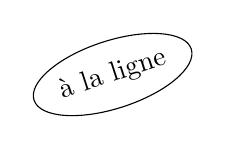
\begin{tikzpicture}[baseline]
\draw[rotate=18] (0,0) ellipse (1.05 and .43);
\node[rotate=18] at (0,0) {à la ligne};
\end{tikzpicture}}}}

\handwritten{\figure{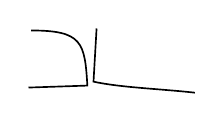
\begin{tikzpicture}[x=.65cm,y=.5cm]
\draw[line width=.6pt] (-1.1,.8) .. controls (-.1,.8) and (-.05,.5) .. (0,-.6) -- (-1.15,-.65);
\draw[line width=.6pt] (.18,.85)--(.12,-.5) .. controls (.65,-.65) and (1.4,-.68) .. (2.1,-.78);
\end{tikzpicture}}}
\inserted{\handwritten{2.7.2.}} U\unsure{\rlap{a}n|\rlap{\raisebox{-.2ex}{n}}n} autre exemple important est celui où les groupes $G_i$ sont finis, de sorte que
\[
G=\underset{\handwritten{\longleftarrow}}{\lim}G_i
\]
est\deleted{\unsure{n|x}} un groupe topologique compact totalement discontinu, ou \handwritten{\uline}{groupe pro\rlap{f}\handwritten{f}ini}. U\unsure{\rlap{a}n|\rlap{\raisebox{-.2ex}{n}}n}e opération de $\handwritten{\underline}{G}$ sur $E$ revient alors à une opération de $G$ sur $E$ qui est continue, ou ce qui revient au même, telle que le stabilisateur de tout point de $E$ est un sous-groupe ouvert de $G$. Le topos classifiant $B_{\handwritten{\underline}{G}}$ sera aussi noté $B_G$, où,bien entendu, $G$ doit être considéré comme muni de sa topologie profinie.

\handwritten{2.7.3.} Il est facile de vérifier,\deleted{que} utilisant les remarques de 2.6, que le topos $B_{\handwritten{\underline}{G}}$ défini par un systême projectif strict \deleted{de} $\handwritten{\underline}{G}=(G_i)_{i\handwritten{\in}I}$ de groupes n'est équivalent à un topos de la forme $\handwritten{\hat}{C}$ que si ce systême projectif est essentiellement constant; dans le cas d'un groupe profini, cela signifie que ce groupe est en fait fini.

